%\documentclass[oneside,final,14pt]{article}
\documentclass[a4paper, 12pt, onecolumn]{extarticle}
%\documentclass[a4paper, 9pt, twocolumn]{extarticle}
\usepackage[T2A]{fontenc}
\usepackage[utf8]{inputenc}
\usepackage[english, russian]{babel}
\usepackage{vmargin}
\usepackage{amsmath}
\usepackage{amsthm}
\usepackage{graphicx}
%\linespread{1.5}
%\setpapersize{A4}
\setmarginsrb{1.5cm}{2cm}{1.5cm}{1cm}{0pt}{0mm}{0pt}{0mm}
\usepackage{indentfirst}
\usepackage{titlesec}
\usepackage{cite}
\usepackage[dvipsnames]{xcolor}
%\titleformat{\section*}[block]{\normalfont\large\bfseries\centering}{\thesection}{1ex}{}
\usepackage[margin=9pt,labelsep=period,font=small,figurename=Fig.]{caption}
%\usepackage[export]{adjustbox}
\usepackage{enumerate}
\usepackage{multirow}
%\setlength{\mathindent}{0\parindent}
%\setlength{\parindent}{0cm}
\sloppy
\setcounter{secnumdepth}{4}
\begin{document}
%\renewcommand{\thesection}{\arabic{section}.}
%\renewcommand{\thesubsection}{\arabic{section}.\arabic{subsection}}
%\renewcommand{\theparagraph}{}
\newtheorem{theorem}{Theorem}
\author{Vyacheslav A. Trofimov\textsuperscript{1}, Dmitry M. Kharitonov\textsuperscript{2}, Mikhail V. Fedotov\textsuperscript{2}}
\title{THG based on induced cubic non-linear processes  due to cascading SHG}

\date{\textsuperscript{1} South China University of Technology, Guangzhou 510641, China\\
\textsuperscript{2}Lomonosov Moscow State University, Leninskye Gory, Moscow 119992, Russia}
\maketitle
% \begin{large}
% \centerline{Lomonosov Moscow State University, Leninskye Gory, Moscow 119992, Russia}
% \end{large}
\section*{Abstract}

As well-known, a problem of the effective THG is of interest because of its wide application. Till present time, the highest efficiency of frequency tripling is achieved by using  consecutive generation of  the SHG and a wave with the sum frequency using two crystals with the quadratic nonlinear response. 

We propose to use the cascading SHG for manifestation of the frequency conversion processes inherent a medium, possessing cubic susceptibility. Based on multi-scale method, the modified equations describing frequency tripling process are derived from a set of the  Schr\"{o}dinger equations describing three-waves interaction with the frequencies  \(\omega,\,2\omega,\,3\omega\) in a medium with quadratic susceptibility.  The derived equations are solved analytically in the frame-work of long pulse  duration approximation and plane wave approximation without using the fundamental wave energy non-depletion approximation. An achievement of THG efficiency being equal to $94.5\%$ is demonstrated. A possibility of highly intense THG is shown for both cases of the phase mismatching between second harmonic and fundamental wave. Choice of its sign allows one to avoid developing modulation instability. Analytical solution is confirmed by computer simulation results.

\section*{Introduction}
The cascaded \(\chi^{(2)}\) nonlinear phenomenon remains of interest for many years due to its various practical applications. For the first time, this phenomena has been theoretically predicted in 1974 by A.P. Sukhorukov and Yu.N. Karamzin \cite{bib:n1}. Since 1991 there is a permanent interest \ to this phenomenon. So, in 1994, a physical experiment was made by a group of Torruellas \cite{bib:n2}. Then, many researchers have predicted and observed various types of cascading \(\chi^{(2)}\) solitons, in particular, 1D spatial \(\chi^{(2)}\) solitons \cite{bib:n3}, and 2D spatial \(\chi^{(2)}\) solitons \cite{bib:n2, bib:n4, bib:n5}, and \(\chi^{(2)}\) temporal solitons \cite{bib:n6}, and spatio-temporal solitons\cite{bib:n7} and others \cite{bib:n9,bib:n10}. Paper \cite{bib:n8}, for example, contains the comprehensive review of observing the cascading \(\chi^{(2)}\) solitons and their practical applications. 

One of the cascading SHG applications is the soliton compression \cite{bib:n11, bib:n12, bib:n13, bib:n14, bib:n15, bib:n16, bib:n17, bib:n18}. By choosing the appropriate sign of the phase mismatching, the pulse compression at the fundamental frequency (FF) can be reached. This phenomenon is also of interest nowadays. So, in \cite{bib:n11}, a soliton compression factor about of \(173.52\) is achieved. M. Bache and F.W. Wise have discussed in \cite{bib:n12} the soliton compression at the wavelength \(1030\,nm\) in a LiNbO$_3$ crystal, which length being equal to \(10\,cm\). In \cite{bib:n13} the pulse compression is obtained at the incident pulse with peak power density \(20\,GW/cm^2\). In \cite{bib:n14} such a pulse compression is observed BBO crystal with its length about of \(3\,cm\). 


Big phase mismatching between waves at the FF and the doubled frequency may lead to self-focusing or defocusing of the beam at the FF, as it was shown in \cite{bib:n19}. In the axial-symmetric case, the beam intensity may be increased about 70 times \cite{bib:n20}. Another important application of the cascading SHG is its using for suppressing random fluctuations of both duration and  maximal power density of pulses generated by  laser operating in the so-called free-generation mode \cite{bib:n21,bib:n22,bib:n23a,bib:n23}  because a frequency conversion of these sub-pulses possesses a low efficiency arising from fluctuations of their maximal intensity. We stress that only about \(2\%-3\%\) of the incident energy is lost  at suppressing those fluctuations.

Thus, observing of phenomena inherent in  the Kerr effect in a medium with the quadratic susceptibility at the cascading SHG (for brevity, we will name this as induced cubic non-linearity or susceptibility) was in many papers. Herewith, all authors mentioned above have taken into account the phase self-modulation only for the laser pulse at the FF. However, cascading SHG induces a response similar cubic susceptibility and it may  lead to THG if the corresponding phase matching occurs. Indeed, let us suppose that the incident fundamental wave (FW) intensity is high enough for manifesting the quadratic nonlinear response of a medium but not remarkable for manifesting of effects corresponding to the third-order susceptibility. At a big phase mismatching between waves with the doubled frequency and FF, the SH intensity remains low, but  THG (\(\omega_3=3\omega\)) may be observed if the phase matching between FW and a wave at trebled frequency occurs.

To evaluate the proposed method of the frequency trebling, it is necessary to discuss available  well-known modern schemes of the THG. There are some ways for achieving  high efficient THG. The most common way consists in a scheme with two nonlinear crystals. The first one is used for the phase-matched SHG, and the second one -  for a phase-matched sum frequency wave generation (SFG).  Using this scheme, the conversion efficiency, being equal $80\%$,  is achieved in physical experiments  \cite{bib:t4a,bib:t4}. For this aim, two Type II KDP crystals were used, each $70\, mm$ diameter and 12 mm thick, polished to a flatness of
$\lambda/4$ at $0.5\mu m$ with a wedge of 7 arcsec.  Another technique of the trebled frequency  generation is based on using Quasi-Periodic Optical Superlattice (QPOS) \cite{bib:t2}.   The maximum frequency conversion achievable in this generation schemes is about $30\%$-$40\%$.

High-efficient THG (about $40\%$ ) can also be achieved in a single crystal \cite{bib:t3}  The FW pulse with duration  $40\,ps$ and a beam  diameter $10\,mm$ falls on the nonlinear crystal ( $20\,mm \cdot 20\,mm \cdot 10\,mm $ KDP crystal, for definiteness), in which the SH is generated. The FW  energy is changed  from $0.5$ to $4.5\,mJ$. Then, a quarter-wave plate is used for changing SH wave polarization: this is necessary for achieving  phase matching at SFG process. After that, the  FW and SH waves, passed through the crystal,  are reflected by the mirror and propagate in the same crystal, in which the THG occurs.  We stress that the beam with enough big diameter is used in this experiment to avoid an influence of its diffraction.  

THG is realized also in a single BBO crystal with combined (quadratic and cubic) nonlinear response  \cite{bib:t1}, in which the phase matching for the frequency tripling occurs, and the SHG and SFG processes occur without phase matching. However, there are some peculiarities that differs this paper from our current paper. So, the incident pulse power density is enough high (\(50\,GW/cm^2\) and higher). Therefore, the third order susceptibility influences the frequency conversion process. It results in presence of cross- and self phase-modulation of optical pulse that is limiting the THG efficiency.  The  frequency trebling based on our scheme allows us to compensate partly a negative influence of the self- and cross-modulation caused by own third order susceptibility because of cascading processes. 

It is necessary to emphasize that the BBO crystal length in those physical experiments is equal to \(1\,mm\), which is too small to observe a high efficiency of THG in our case under consideration. We also note that the theoretical analysis was provided in the framework of the FW intensity non-depletion approximation. In turn, we propose a new approach for theoretical analysis, which is free of this approximation. 

In frequency conversion scheme proposed below is used one nonlinear crystal with quadratic nonlinear response. However, in  contrast to \cite{bib:t4} the changing  electric field polarization at the SH wave is not required because we need only the phase matching between TH and FW. The SH intensity is very low (about $2\%$ - $3\%$ or less that is comparable with losses at the mirror \cite{bib:t4a,bib:t4}) and the FW energy converts mostly to TH one. Secondly, our scheme can be applied directly for femtosecond pulses without a synchronization between  FW and SH \cite{bib:t5}, where a time pre-delayer was used to compensate the group velocity mismatching (GVM) between FW and SH. 

While the two-crystal scheme requires the ideal ratio between the FW and SH intensities in the input section of the second crystal (it must be equal to ratio as $1:2$), our scheme is free from this demand. THG based on cascading mechanism  allows on to observe thee its high efficiency even for rather low intensity (about \(1\,GW/cm^2\) and low) of the incident pulse at FF with big duration: picosecond or  nanosecond or  even microsecond duration to minimize an  influence of the GVM  and the second-order dispersion (SOD) on the frequency up-conversion because the induced cubic susceptibility is much greater than the own susceptibility of the third order.
Because  the THG based on cascading SHG accompanies by  cross -modulation of the trebled frequency that leads to broadening of its spectrum. Therefore, one can additionally compress of the pulse. In the scheme using only quadratic nonlinear response, such a possibility is absent.  On the other hand, the terms in equations responsible for the pulse broadening of TH spectrum  differ from those occurring in a medium with own third order susceptibility. 

Our paper is organized as follows. We start from the set of Schr\"{o}dinger equations, which describes three-waves  interaction (FW, SH and TH) in a medium with quadratic and cubic non-linear response. Let's notice that the accounting for cubic non-linearity is used only for proving of inducing  cubic susceptibility in a medium with quadratic non-linear response due to the cascading SHG. The last  process is mainly attracted our attention, and,  we demonstrate an appearance of induced  cubic susceptibility  on the base of multi-scale method (see, for example, \cite{bib:n24}) similar to that presented in \cite{bib:n19}. Then we prove it  by testing  several cases of waves-interaction.  With this aim, the analytical solution of the modified problem, obtained by using multi-scale method, is derived. An influence of the phase mismatching between interacting waves on the THG efficiency is examined  theoretically in long pulse duration approximation.

The computer simulation is made in the last part of the paper. So, firstly,  the analytical solution is confirmed without accounting for SOD of the pulses. Then, the THG efficiency  of pulses undergoing SOD  influence is analyzed. Developing of the MI is analyzed by computer simulation in Supplementary Information. 

\section*{PROBLEM STATEMENT}

To clarify our scheme of the frequency trebling let us consider the following frequency conversion processes, depicted schematically in Fig. \ref{fr:match} for a crystal with quadratic (\(\chi^{(2)}\)) and cubic (\(\chi^{(3)}\))  susceptibilities. A  symbol \(\omega\) denotes  the FW frequency. Thus, we consider three processes producing a wave with trebled frequency. 

First process is a generation of an optical wave with doubled frequency (\(\omega+\omega=2\omega,\,\chi^{(2)}\)), and simultaneously THG based on the SFG (\(\omega+2\omega=3\omega,\,\chi^{(2)}\)) due to quadratic non-linear response of a crystal. The second one is directly the trebled frequency wave generation \(\chi^{(3)}_{cas}\)   due to cubic non-linearity of a crystal. In comparison with the frequency doubling process this process requires  more intensive  incident pulse. The third (new) process of the frequency tripling is based on the frequency doubling at big mismatching, and this process can occur at low intensity of the incident wave in comparison of those occurring at own cubic non-linearity of a crystal. This process is denoted as \(\omega\rightarrow3\omega\) with symbol \textcolor{red}{ \(\chi^{(3)}_{cas}\)} \textcolor{ForestGreen}{$\chi^{(3)}$}. In Fig. \ref{fr:match} we also depict another frequency conversion processes (\(3\omega=2\omega+2\omega-\omega,\,\chi^{(3)}\)), which is taken into account by us. Each of these frequency conversion processes is accompanied by own phase matching and own value of crystal susceptibility at the corresponding frequencies. Therefore, the susceptibilities \(\chi^{(3)}\) and  \(\chi^{(3)}_{cas}\) are different. As a rule, only one of various conversion processes can occur at phase matching: in Fig. \ref{fr:match} this process is THG ($\chi^{(3)}$).
\begin{figure}[h!]
\centering
\includegraphics[width=0.4\textwidth]{Matching2}
\caption{Scheme of the phase matching and mismatching for various processes of frequency conversion.}
\label{fr:match}
\end{figure}
We suppose that the angle range for achieving the phase matching of the corresponding generation process is small enough to avoid its overlapping with phase matching angle range of other processes. In this case, it is possible to differ the process of THG, which occurs due to the SFG process, and due to the cascading SHG.

Starting from the Maxwell's equations,  one can derived the following set of dimensionless Schr\"{o}dinger equations with respect to slowly varying envelopes of the wave packets: 
\begin{equation}
\label{eq:ref1}
\begin{aligned}
&\frac{\partial{A_1}}{\partial{z}}+iD_1\frac{\partial^2{A_1}}{\partial{t^2}}+i\left(\gamma_{12} A_1^* A_2e^{-i\Delta_{21} kz}+\gamma_{23} A_2^* A_3e^{-i(\Delta_{31}k-\Delta_{21}k)z}\right)=0,\\
&\frac{\partial{A_2}}{\partial{z}}+\nu_{21} \frac{\partial A_2}{\partial t}+iD_2\frac{\partial^2{A_2}}{\partial{t^2}}+i\left(\gamma_{11}A_1^2e^{i\Delta_{21} kz}+2\gamma_{13}A_1^*A_3e^{-i(\Delta_{31}k-\Delta_{21}k)z}\right)=0,\\
&\frac{\partial{A_3}}{\partial{z}}+\nu_{31} \frac{\partial A_3}{\partial t}+iD_3\frac{\partial^2{A_3}}{\partial{t^2}}+3i\gamma_{21} A_1 A_2e^{i(\Delta_{31}k-\Delta_{21}k)z}=0,\, 0< z \leq L_z , 0<t<L_t\\
\end{aligned}
\end{equation}
which describes the optical frequency tripling in a medium with combined nonlinear response in the frame-work of the plane wave approximation (without taking into account a laser beam diffraction). 
Here \(A_1,\,A_2\) and \(A_3\) are the complex amplitudes of waves with the FF (\(\omega\)), and the doubled frequency (\(2\omega\)), and the tripled frequency (\(3\omega\)), respectively, normalized at \(A_{01}=\sqrt{I_{01}}\) (a square root of the incident pulse maximal intensity at the FF). Parameter \(\gamma_{jk}\) is the interacting waves coupling coefficient  due to the quadratic non-linear response at the corresponding frequencies.  In general case, this coefficient may be different for various generation processes. However, for simplicity, we choose the same value (\(\gamma_{jk}=\gamma\)) for all these processes involving in equations \eqref{eq:ref1}. Parameter \(\Delta_{21} k=k_2 - 2k_1\)  characterizes the phase mismatching on the length $Z_n=1\,mm$ in which units a longitudinal coordinate $z$ is measured. \(k_1\) and \(k_2\), denote dimensionless wave-numbers for waves with the FF and doubled frequency. Parameter \(\Delta_{31} k=k_3 - 3k_1\) characterizes the phase mismatching on $Z_n$ at THG. A symbol \(k_3\) denotes dimensionless TH wave-number. Coordinate \(t\) is a time, measured in units of the pulse duration \(\tau_P\) at the FF. Parameters \(\nu_{21}\) and \(\nu_{31}\) characterize dimensionless GVM between SH and FW, and TH and FW, respectively. Parameters \(D_{j}, j=1,2,3\) characterize dimensionless SOD of the corresponding wave packet. Parameters \(L_t\) and \(L_z\) define the time interval, during which the laser pulse interaction is analyzed, and the maximal distance of the pulse propagation, respectively.

The initial distributions of the complex amplitudes are the following:
\begin{equation}\begin{aligned}
\label{eq:first}
&A_1(0,t)=A_{10}(t),\, A_2(0,t)=0,\,A_3(0,t)=0,\, t\in[0,L_t],\\
\end{aligned}\end{equation}
and corresponds to a finite distribution of the laser pulses.

Let us discuss the terms in the set of the equations \eqref{eq:ref1}. The term \(\gamma A_1^2e^{i\Delta_{21} kz}\) (\(\chi^{(2)}(2\omega;\,\omega,\omega\))) in the second equation corresponds to the generation of a wave with doubled frequency for the process (\(\omega+\omega\rightarrow2\omega\)). The term \(\gamma  A_1^* A_2e^{-i\Delta_{21} kz}\) in the first equation is responsible for the opposite process (\(2\omega \rightarrow \omega+\omega\)). A process of the THG via the SFG is described by the term \(\gamma A_1 A_2e^{i(\Delta_{31}k-\Delta_{21}k)z}\) (\(\chi^{(2)}(3\omega;\,\omega,2\omega\))) in the third equation. In turn, the term \(\gamma A_2^* A_3e^{-i(\Delta_{31}k-\Delta_{21}k)z}\) in the first equation and the term \(\gamma A_1^* A_3e^{-i(\Delta_{31}k-\Delta_{21}k)z}\) in the second equation correspond to the reverse processes (\(3\omega\rightarrow2\omega+\omega\)). 

Let us note that the introduced dimensionless parameters and functions are expressed through the physical ones, denoted with containing line above them, with accordance to a rule:
\begin{equation}
\label{eq:pars}
\begin{aligned}
&A_j=\frac{\bar{A}_j}{\sqrt{I_{01}}},\,D_j=-\frac{1}{2}\frac{\partial^2 \bar{k}}{\partial \bar{\omega}^2}\Big|_{\bar{\omega}_j}\frac{Z_n}{\tau_P^2},\omega_j=\bar{\omega}_j\tau_P,\,j=1,2,3,\,t=\frac{\bar{t}}{\tau_P},\,z=\frac{\bar{z}}{Z_n},\\
&\nu_{j1}=\left(\frac{\partial \bar{k}}{\partial \bar{\omega}}\Big|_{j\bar{\omega}}-\frac{\partial \bar{k}}{\partial \bar{\omega}}\Big|_{\bar{\omega}}\right)\frac{Z_n}{\tau_P},\,\Delta_{j1}k=\Delta_{j1}\bar{k}Z_n,\,j=2,\,3\\
&\gamma=\frac{2\pi\chi^{(2)}\bar{k}\sqrt{I_{01}}}{n^2}Z_n,
\end{aligned}
\end{equation}
$n$ is a refractive index at FF.

For computer simulation we choose the following values of the physical parameters: \(\tau_P \text{ is changed from } 100fs\text{ to }10ps,\) the wavelength corresponding to wave with FF is equal to \(\lambda_1=1064\,nm\) or \(\lambda_1=800\,nm\).  The angle \(\theta\) of the phase matching for the THG, and the second order susceptibility of selected crystals with dependent on the angles \(\theta\) and \(\varphi\) as well as the incident pulse intensity, at which the coupling coefficient \(\gamma\) is equal to unity at the phase matching angle \(\theta\) and the crystal length $1\,mm$, are shown in Table \ref{tab:2}. The angles are measured between the crystal axis in the uni-axial crystal and wave vector of the FW.We also show the references to the papers, which contain the data, after the names of the crystals.

\begin{table}[h]
\caption{The second order susceptibility of some crystals and the incident pulse intensity $I_0$ in dependence of the laser pulse propagation direction with respect to the crystal axis: \((\theta,\,\varphi)\) are spherical coordinates. Phase matching angles are provided for FW length $\lambda=1064\,nm$. }
{\begin{tabular}{|c|c|c|c|} 
\hline
Crystal& THG matching angle $\theta (^{\circ})$& $\chi^{(2)} (pm/V)$ & $ I_0\,(10^9\,W/cm^2)$ \\
\hline
KDP \cite{bib:n26,bib:c4}& 64.97 & $0.76\sin\theta\sin(2\varphi)$ & 2 \\
\hline
ADP \cite{bib:n26,bib:c4}& 66.58& $0.76\sin\theta\sin(2\varphi)$ & 2.03 \\
\hline
BBO \cite{bib:c1,bib:c4}& 37.48& $4.32(\sin\theta-0.07\cos\theta\sin(3\varphi))$ & 0.21 \\
\hline
KBBF \cite{bib:c2,bib:c5}& 31.16& $0.98\cos\theta\cos(3\varphi)$ & 1.28 \\
\hline
RBBF \cite{bib:c3}&33.77& $0.9\cos\theta\cos(3\varphi)$ & 1.63 \\
\hline
\end{tabular}
\label{tab:2}}
\end{table}


The frequency conversion efficiency is estimated as:
\begin{equation}
\eta_j(z)=\frac{\int\limits_0^{L_t}|A_j(z,t)|^2dt}{\int\limits_0^{L_t}|A_1(z=0,t)|^2dt}.
\end{equation}
Another characteristic, which describes the frequency conversion process, is the pulse spectra. They are computed by the formula
\begin{equation}
\hat{A}_j^\omega(z;\omega)=\frac{1}{\sqrt{2\pi}}\int\limits_{0}^{L_t} A_j(z,t)e^{-i\omega t}dt,\,j=1,\,2,\,3
\end{equation}
using the NumPy module \cite{bib:np} of Python Language. 

The set \eqref{eq:ref1} of equations  possesses some invariants:
\begin{equation}
\label{eq:inv1}
\begin{aligned}
&I_1=\int\limits_0^{L_t}\left(|A_1|^2+|A_2|^2+|A_3|^2\right)dt\\
\end{aligned}
\end{equation}
--the first invariant (the energy preservation law),
\begin{equation}
I_2=\int\limits_0^{L_t}\left(\sum\limits_{j=1}^3 p_j A_j \frac{\partial A_j^*}{\partial t}\right)dt,\,p_1=6,\, p_2=3,\, p_3=2
\end{equation}
--the second invariant,
\begin{equation}
\label{eq:inv3}
\begin{aligned}
&I_3=\int\limits_0^{L_t}\Big(-\sum\limits_{j=1}^3 p_jD_j |\frac{\partial A_j}{\partial t}|^2-p_2\nu_{21}Im\left(A_2^*\frac{\partial A_2}{\partial t}\right)-p_3\nu_{31}Im\left(A_3^*\frac{\partial A_3}{\partial t}\right)+6\gamma Re\bigl(2A_1 A_2 A_3^*e^{i(\Delta_{31}k-\Delta_{21}k)z}\\
&+A_1^2 A_2^*e^{\Delta_{21}k\cdot z}\bigr)+3\Delta_{21} k|A_2|^2+2\Delta_{31} k|A_3|^2\Big)dt,
\end{aligned}
\end{equation}
-- the third invariant (Hamiltonian). At this invariant derivation, firstly the substitution $A_j=\bar{A}_j\exp(i\Delta_{j1}kz),\,j=2,\,3$and secondly, inverse transform to the functions $A_j$ were used.

Let us notice that  the integration limits change on \(\{-\infty,\infty\}\), respectively if the laser pulse interaction is analyzed in unbounded time domain. 

\section*{Induced cubic non-linear processes based on cascading SHG}

\subsection*{Derivation of the modified  equations}
For simplicity of  analysis at deriving equations describing THG, let's make a substitution of TH complex amplitude as follows:
$$
{A}_3=\bar{A}_3e^{i\Delta_{31}kz}
$$
(for brevity, the bar is omitted below ). The equation set \eqref{eq:ref1} is transformed to the form
\begin{equation}
\label{eq:refg}
\begin{aligned}
&\frac{\partial{A_1}}{\partial{z}}+iD_1\frac{\partial^2{A_1}}{\partial{t^2}}+i\gamma\left(A_1^* A_2e^{-i\Delta_{21} kz}+A_2^* A_3e^{i\Delta_{21}kz}\right)=0,\\
&\frac{\partial{A_2}}{\partial{z}}+\nu_{21}\frac{\partial A_2}{\partial t}+iD_2\frac{\partial^2{A_2}}{\partial{t^2}}+i\gamma\left(A_1^2e^{i\Delta_{21} kz}+2A_1^*A_3e^{i\Delta_{21}kz}\right)=0,\\
&\frac{\partial{A_3}}{\partial{z}}+\nu_{31}\frac{\partial A_3}{\partial t}+iD_3\frac{\partial^2{A_3}}{\partial{t^2}}+3i\gamma A_1 A_2e^{-i\Delta_{21}kz}+i\Delta_{31}kA_3=0,\,0< z \leq L_z , 0<t<L_t.\\
\end{aligned}
\end{equation}

As we mention above, quadratic susceptibility in cascading limit leads to appearance of induced cubic nonlinear response. It is easy to show, using multi-scale method \cite{bib:n24}. Because the derivation is rather complicated, we place it in Appendix. Here we present the final result: complex amplitudes $A_j,\,j=1,\,2,\,3$ can be approximated with the precision of $O(\Delta_{21}k^{-2})$: 
\begin{equation}
\label{eq:exp3}
\begin{aligned}
&A_1=U, A_2=\frac{1}{\Delta_{21}k}(-\gamma (U^2+2U^*W)e^{i\Delta_{21}kz}+v_1), A_3=We^{i\Delta_{31}kz},\\
\end{aligned}
\end{equation}
where functions \(U,\,W,\,v_1\) are governed by the set of nonlinear equations:
\begin{equation}
\label{eq:main2}
\begin{aligned}
&\frac{\partial U}{\partial z}+iD_1\frac{\partial^ U}{\partial t^2}-i\frac{\gamma^2}{\Delta_{21} k}(|U|^2U+3U^{*2}W+2U|W|^2)=0,\\
&\frac{\partial W}{\partial z}+\nu_{31}\frac{\partial W}{\partial t}+iD_3\frac{\partial^2 W}{\partial t^2}-3i\frac{\gamma^2}{\Delta_{21} k}(U^3+2|U|^2W)+i\Delta_{31}kW=0,\,\frac{\partial v_1}{\partial t}+\nu_{21}\frac{\partial v_1}{\partial t}+iD_2\frac{\partial^2 v_1}{\partial t^2}=0\\
\end{aligned}
\end{equation}
with the following initial conditions:
\begin{equation}
\label{eq:ini2}
U|_{z=0}=A_{10}(t),\,W|_{z=0}=0,\,v_1|_{z=0}=\gamma A_{10}^2(t).
\end{equation}
and zero-valued BCs because all pulses have finite initial distribution and we consider bounded domain in \(z\)-coordinate. We call below the problem \eqref{eq:main2}-\eqref{eq:ini2} as the modified problem.

The first two equations \eqref{eq:main2} can be obtained in much more simple way. For this, we use the following representation of the complex amplitude $A_2$:
$$
A_2=(A_2^{(0)}+A_2^{(1)}+A_2^{(2)}+...)e^{i\Delta_{21}kz}.
$$
Insert this series into the second equation \eqref{eq:refg}. Then, we obtain the following equation in the first approximation:
$$
\frac{\partial A_2^{(0)}}{\partial z}+\nu_{21}\frac{\partial A_{2}^{(0)}}{\partial t}+iD_2\frac{\partial A_2^{(0)}}{\partial^2 t^2}+i\Delta_{21}kA_2^{(0)}+i\gamma(A_1^2+2A_1^*A_3)=0,
$$
which can be rewritten as
$$
A_2^{(0)}+\frac{\gamma}{\Delta_{21}k}(A_1^2+2A_1^*A_3)-\frac{i}{\Delta_{21}k}\frac{\partial^2 A_2^{(0)}}{\partial z}+\frac{\nu_{21}}{\Delta_{21}k}\frac{\partial A_{2}^{(0)}}{\partial t}+i\frac{D_2}{\Delta_{21}k}\frac{\partial A_2^{(0)}}{\partial t^2}=0.
$$
One can see that last two terms contain both complex amplitude $A_2^{(0)}$ and $\Delta_{21}k^{-1}$. Therefore, they are much smaller than other terms, so can be neglected. So, we obtian the following relation:
\begin{equation}
\label{eq:ap_exp}
A_2^{(0)}=-\frac{\gamma}{\Delta_{21}k}(A_1^2+2A_1^*A_3).
\end{equation}
The terms in the right part describe phase gratings, induced at doubled frequency, where $A_1^2$ will lead to THG and FW self-modulation; $2A_1^*A_3$ will lead to cross-modulation between waves and to reverse energy conversion from TH to FW. Substitute now the representation \eqref{eq:ap_exp} into the first equation and the third equation \eqref{eq:refg}:
$$
\begin{aligned}
&\frac{d{A_1}}{d{z}}+i\frac{\gamma^2}{\Delta_{21} k}(-|A_1|^2U-3A_1^{*2}A_3-2A_1|A_3|^2=0,\\
&\frac{d{A_3}}{d{z}}-3i\frac{\gamma^2}{\Delta_{21} k}(A_1^3+2|A_1|^2A_3)+i\Delta_{31}kA_3=0,
\end{aligned}
$$
which correspond with the first two equations \eqref{eq:main2}. It should be noted that this approach is not as flexible as the multi-scale method. For example, the representation \eqref{eq:ap_exp} does not satisfy the initial condition. On the other hand, this allows us to give some physical background of the discussed problem.

Nevertheless, the equations  \eqref{eq:main2} possess the energy conservation law: 
\begin{equation}
\label{eq:ninv1}
I_1=\int\limits_0^{L_t}\left(|U|^2+|W|^2\right)dt=const
\end{equation}
if the functions \(U,\,W\) are equal to zero at the time moments \(t=0,L_t\).  

The Hamiltonian of the equation set \eqref{eq:main2} is written in the form:

\begin{equation}
\label{eq:ninv3}
\begin{aligned}
I_3&=\int\limits_0^{L_t}\Big(2\nu_{31}Im\left(W^*\frac{\partial W}{\partial t}\right)-6D_1|\frac{\partial U}{\partial t}|^2-2D_3|\frac{\partial W}{\partial t}|^2-\\
&\frac{3\gamma^2}{\Delta_{21}k}\left(4Re(U^3W^*)+|U|^4+4|U|^2|W|^2\right)+2\Delta_{31}k|W|^2\Big)dt=const.
\end{aligned}
\end{equation}

We  emphasize that a value of the energy invariant \eqref{eq:ninv1} coincides with a value of  \eqref{eq:inv1} because these invariants are equal to \(\int\limits_0^{L_t}|A_{10}|^2dt\). However, because the invariant for the  set modified equations do not contain the SH wave, then the sum energy of two other waves will be greater than a sum of the energies of corresponding waves computed using the original problem.

It should be told a few words about physical mechanism of appearance of  non-linear processes inherent cubic non-linearity at the laser pulse propagation in a medium with quadratic non-linear response under the cascading SHG. For example, in  \cite{bib:n19} the authors stress that the self-lensing term $|A|^2A$, which describes the nonlinear phase shift acquired during sequences of cascaded photon processes, each involving upconversion to $2\omega$ followed by backconversion at $\omega$. This two-step process leads to an effective cubic susceptibility $\chi_{eff}^{(3)}(\omega; \omega,2\omega,\omega) \leftarrow \chi^{(2)}(\omega; 2\omega,2\omega)\chi^{(2)}(2\omega; \omega,\omega)$, which is characteristic of the effective four-photon interaction $\omega=\omega-\omega+\omega$. But in this paper as well in many another papers, the authors consider only the first two equations in \eqref{eq:refg} with respect FW and SH. If the phase mismatching $\Delta_{21}k$ is big then the SH complex amplitude is proportional to $A_1^2$. It means that the response of a medium  contains of phase grating  on the frequency $2\omega$. The optical radiation with FW scatters on the grating and the TH appears. If the phase matching for TH and FW occurs then this process will be significant. But early the researchers have paid attention only to problem of the self- (or de-) compression (or soliton formation) of the laser pulse  under the cascading SHG and did not discuss its possible using for frequency up-conversion. Mathematically, we can see a term responsible THG if we analyze all three equations in \eqref{eq:refg} and put instead a small amplitude $A_2$ the term  $A_1^2$ in the third equation. This is rough mathematical reasoning. Correct math expression is derived on the base of multi-scale method. 

\subsection*{Exact solution of the modified problem.}
In the framework of the long pulse duration approximation, the functions \(U,W\) depend only on \(z\) coordinate, and we can rewrite the problem \eqref{eq:main2},\eqref{eq:ini2} in the form:
\begin{equation}
\label{eq:main2l}
\begin{aligned}
&\frac{dU}{dz}-i\frac{\gamma^2}{\Delta_{21} k}(|U|^2U+3U^{*2}W+2U|W|^2)=0,\\
&\frac{dW}{dz}-3i\frac{\gamma^2}{\Delta_{21} k}(U^3+2|U|^2W)+\Delta_{31}kW=0,\,  0< z \leq L_z\\
&U(0)=1,\,W(0)=0.\\
\end{aligned}
\end{equation}
The invariants \eqref{eq:ninv1}, \eqref{eq:ninv3} are written as follows:
\begin{equation}
\label{eq:ninvs}
\begin{aligned}
&I_1=|U|^2+|W|^2,\\
&I_3=\frac{\gamma^2}{\Delta_{21}k}\left(-12Re(U^3W^*)-3|U|^4-12|U|^2|W|^2\right)+2\Delta_{31}k|W|^2.
\end{aligned}
\end{equation}
We note that the first invariant of the problem \eqref{eq:main2l} equals unity (\(I_1=1\)) due to the initial conditions.

To write intensities evolution for the interacting waves, we use a well-known representation for the complex amplitudes:
\begin{equation}
\label{eq:repr}
U(z)=a_1e^{i\varphi_1(z)},\,W(z)=a_3e^{i\varphi_3(z)},
\end{equation}
where \(a_j,\,\varphi_j\) are the real functions describing amplitudes and phases of the waves. In new notations, the equations \eqref{eq:main2l} are re-written:

\begin{equation}
\label{eq:main3}
\begin{aligned}
&\frac{da_1}{dz}=-\frac{3\gamma^2}{\Delta_{21}k}a_1^2a_3\sin\varphi,\\
&\frac{da_3}{dz}=\frac{3\gamma^2}{\Delta_{21}k}a_1^3\sin\varphi,\\
&\frac{d\varphi}{dz}-\frac{3 \gamma^2}{\Delta_{21}k}\left(a_1  \left(\frac{a_1^2}{a_3}-3a_3\right)\cos\varphi+a_1^2-2a_3^2\right)+\Delta_{31}k=0,
\end{aligned}
\end{equation}

here \(\varphi=\varphi_3-3\varphi_1\) is a phase difference between TH and FW. The invariants  \eqref{eq:ninvs} are transformed to the following form:
\[
\begin{aligned}
&I_1=a_1^2+a_3^2=1,\\
&I_3=\frac{\gamma^2}{\Delta_{21}k}\left(-12a_1^3a_3\cos\varphi-3a_1^4-12a_1^2a_3^2\right)+\Delta_{31}ka_3^2.
\end{aligned}
\] 

To express \(\cos \varphi\) we modify the third invariant:
\[
\tilde{I}_3=I_3+3\frac{\gamma^2}{\Delta_{21}k}I_1^2=-12\frac{\gamma^2}{\Delta_{21}k}a_1^3a_3\cos\varphi-6\frac{\gamma^2}{\Delta_{21}k}a_1^2a_3^2+3\frac{\gamma^2}{\Delta_{21}k}a_3^4+2\Delta_{31}ka_3^2=0,
\]
which equals zero because the TH incident intensity is equal to zero: \(a_3(0)=0\). Hence, we can express \(\cos \varphi\):
\begin{equation}
\label{eq:cos}
\cos\varphi=\frac{a_3(-6a_1^2+3a_3^2+2q)}{12a_1^3},
\end{equation}
where the parameter $q$ is defined as:
$$
q=\frac{\Delta_{21}k\Delta_{31}k}{\gamma^2},
$$
which characterizes relation between phase incursions because of phase mismatching between SH and FW, and TH and FW, respectively, and because of nonlinear coupling coefficient ${\gamma}$.
Obviously, an inequality 
\[
|\cos\varphi|\le1
\]
must be valid. This leads to restriction on the intensities changing.
Then we find \(\sin \varphi\) from the equality \eqref{eq:cos} and substitute it into the second equation of \eqref{eq:main3}, which is preliminary multiplied by \(a_1\). As a result, we write the following equation with respect to the TH intensity:
\[\frac{da_3^2}{dz}=\pm6\frac{\gamma^2}{\Delta_{21}k}a_1^3a_3\sqrt{1-\frac{a_3^2(-6a_1^2+3a_3^2+2q)^2}{144a_1^6}}.\]
Using the new variable \(p_3=a_3^2\) and expressing \(a_1^2\) from the first invariant \(a_1^2=1-p_3\), we finally obtain:
\begin{equation}
\label{eq:main4}
\begin{aligned}
&\frac{dp_3}{dz}=\pm7.5\frac{\gamma^2}{\Delta_{21}k}\sqrt{p_3f(p_3)},\\
&f(p_3)=\frac{16}{25}((1-p_3)^3-\frac{1}{144}p_3(9p_3+2q-6)^2).
\end{aligned}
\end{equation}
Sign in the right side of the equation corresponds to different processes: sign ``plus" corresponds to a conversion of the FW energy to TH energy, and sign ``minus" to reverse energy conversion from the wave with trebled frequency to the FW. So, since TH incident intensity equals zero, then we choose the sign ``plus".

The intensity evolution is defined by the parameter $q$ because it defines the number of real roots of the equation
$$
f(p_3)=0,
$$
which can be found, for example, by using the Sturm theorem. We  denote them as
$P_{31},\,P_{32},\,P_{33}$, where $P_{31}$ is  real always. If two other roots are also real then we support that there is inequality:   $P_{31}\le P_{32}\le P_{33}$ between them. Obviously, this   assumption does not restrict our consideration.
It should be also stressed that a solution of the equation \eqref{eq:main4} is expressed through the elliptical functions or, in certain cases, through elementary functions. Below we briefly discuss the problem  solution corresponding to various values of the parameter $q$.
Moreover, we вdevelop also the TH phase evolution. Because of the complexity of the obtained formula we do not write it here. However, using the formulas with respect to the phase and the intensity, it is possible to approximate the solution of the problem \eqref{eq:ref1}-\eqref{eq:first} with good accuracy. We show it below using the computer simulation results.

\paragraph*{Domain  $q<-1.5,\,q>3 + \frac{9}{\sqrt[3]{2}}-9\sqrt[3]{ 2}$: two complex roots $P_{32},P_{33}$.}
Only the root $P_{31}$ is positive. As a result, the TH intensity  $p_3(z)$ changes between zero and $P_{31}$ with accordance of the following formula:
\begin{equation}
\label{eq:p1_1}
p_3(z)=|A_3(z)|^2=\frac{cP_{31}(1-cn(7.5\frac{\gamma^2}{\Delta_{21}k}\kappa z,m))}{(d-c)cn(7.5\frac{\gamma^2}{\Delta_{21}k}\kappa z,
m)+(c+d)},
\end{equation}
where
$$
\begin{aligned}
&c=\sqrt{r^2+s^2},\, d=\sqrt{(p_{31}-r)^2+s^2}, \kappa=\sqrt{cd}, m=\frac{\kappa^2+(r+P_{31})r-s^2}{2\kappa^2},\\
&r=Re(P_{32}),\, s=Im (P_{32}).
\end{aligned}
$$
This domain of the parameter $q$ contains important case of THG corresponding to the phase matching between FW and TH ($\Delta_{31}k=0$). Under this condition there is only a unique branch of the TH intensity changing between \(0\) and $P_{31}=0.8$. Other two roots are defined by a solution of the equation \(5p_3^2-8p_3+4=0\), and they are the complex ones (\(P_{31,\,32}=0.8\pm0.4i\)). 
As a result, the TH intensity evolution  is described by:

\begin{equation}
\label{eq:sol}
p_3(z)=\frac{4(1-cn(\frac{3\sqrt[4]{5}\gamma^2}{\Delta_{21}k}z; 0.5(1-\frac{1}{\sqrt{5}})))}{(5+\sqrt{5})-(5-\sqrt{5})cn(\frac{3\sqrt[4]{5}\gamma^2}{\Delta_{21}k}z; 0.5(1-\frac{1}{\sqrt{5}}))}.
\end{equation}
As follows from \eqref{eq:sol}, the coupling coefficient \(\gamma\) and the phase mismatching between FW and SH (\(\Delta_{21}k\))  influence only on the intensity oscillation period. Let's note that in all other modes (at $\Delta_{31}k\ne0$) of THG there is more complicated dependencies of the TH maximal intensity and period  from $\Delta_{21}k$. Therefore, we do not discuss this below. 

\paragraph*{Domain $-1.5<q<3 + \frac{9}{\sqrt[3]{2}}-9\sqrt[3]{ 2}$: three real roots.} 
In this case all three roots $P_{3j}$ are positive. Therefore, there are two regimes of the waves interaction: low-efficient mode and high-efficient one. In low-efficient regime, the TH intensity changes between $0$ and $P_{31}$ as follows:  

\begin{equation}
\label{eq:p1_2}
\begin{aligned}
&p_3(z)=\frac{P_{31}P_{33}sn^2(3.75\frac{\gamma^2}{\Delta_{21}k}\sqrt{P_{32}(P_{33}-P_{31})}z,m)}{P_{31}sn^2(3.75\frac{\gamma^2}{\Delta_{21}k} \sqrt{(P_{32})(P_{33}-P_{31})}z,m)+(P_{33}-P_{31})},\\
&m=\sqrt{\frac{P_{31}(P_{33}-P_{32})}{P_{32}(P_{33}-P_{31})}}.
\end{aligned}
\end{equation} 
In high-efficient regime, the TH intensity changes between values of the roots $P_{32}$ and $P_{33}$ according to the rule:
\begin{equation}
\label{eq:p1_2bis}
\begin{aligned}
&p_3(z)=\frac{P_{32}P_{33}}{(P_{33}-P_{32})sn^2(3.75\frac{\gamma^2}{\Delta_{21}k}\sqrt{P_{32}(P_{33}-P_{31})}z,m)+P_{32}}\\
\end{aligned}
\end{equation}
with the same coefficient $m$ as in \eqref{eq:p1_2}.

\paragraph*{The first special case $q=-1.5$: $0<P_{31}<P_{32}=P_{33}=1$.}
For this parameter value  $q$, the TH intensity $p_3(z)$  changes again between $0$ and $P_{31}=0.64$. However, the solution is expressed through the cosine function:
\begin{equation}
\label{eq:p1_3}
p_3(z)=\frac{P_{31}(1-\cos(6\frac{\gamma^2}{\Delta_{21}k}\sqrt{1-P_{31}}z))}{-P_{31}\cos(6\frac{\gamma^2}{\Delta_{21}k}\sqrt{1-P_{31}}z)+2-P_{31}}=\frac{8(1-\cos(4.5\frac{\gamma^2}{\Delta_{21}k}z))}{-8\cos(4.5\frac{\gamma^2}{\Delta_{21}k}z)+17}.
\end{equation}


\paragraph*{The second special case $q=3+\frac{9}{\sqrt[3]{2}}-9\sqrt[3]{2}$: $0<P_{31}=P_{32}<P_{33}<1$.}
In this case $q\approx-1.2$ , there are two regimes of the frequency conversion. In both of them (low-efficient and high-efficient), the TH intensity $p_3$ evolution is governed  by:

\begin{equation}
\label{eq:p1_4}
\begin{aligned}
&z(p_3)=\frac{1}{7.5\frac{\gamma^2}{\Delta_{21}k}\sqrt{P_{31}(P_{33}-P_{31})}}\ln\frac{\left(\sqrt{(P_{33}-P_{31})p_3}+\sqrt{P_{31}(P_{33}-p_3)}\right)^2}{|p_3-P_{31}|P_{33}},
\end{aligned}
\end{equation}
where the modulus is expanded with positive sign at high-effective regime: $P_{31}<p_3<P_{33}$, and with negative sign at low-effective regime $0<p_3<P_{31}$.

 From \eqref{eq:p1_4} together with computations of the equation
$ f(p_3)=0$ roots, it is possible to compute the THG maximal efficiency: its value is more than $95\%$ and it is achieved at $q=3+\frac{9}{\sqrt[3]{2}}-9\sqrt[3]{2}$ ( Fig.\ref{fr:cglp}).
\begin{figure}
    \centering
    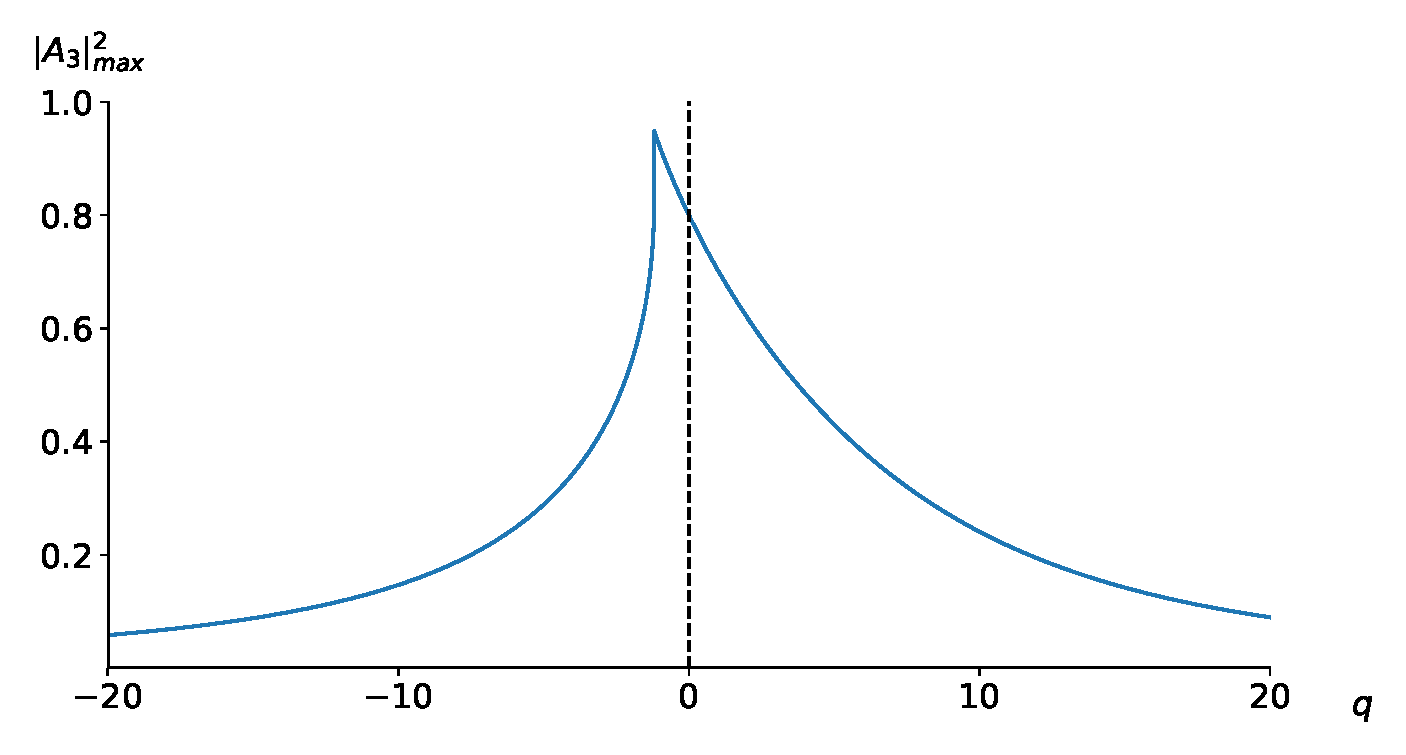
\includegraphics[width=0.8\textwidth]{CGLP_curve.eps}
\caption{Dependence of the TH maximal intensity on the parameter q }
\label{fr:cglp}
\end{figure}
Therefore, the phase matching between TH and FW is not an optimal condition for THG because at $\Delta_{31}k=0$ ($q=0$) only $80\%$ of the FW energy converts to the TH energy.  We see also in  Fig. \ref{fr:cglp} the abrupt decreasing TH maximal intensity near the optimal negative value of the parameter $q$. With increasing positive phase mismatching $\Delta_{21}k$, the negative value of the phase mismatching  $\Delta_{31}k$ tends to zero. Let us note that the efficiency of THG is the same if we change signs of phase mismatches to opposite ones because the value of parameter $q$ does not change at the same time: for example, $\Delta_{21}k=20,\,\Delta_{31}k=-1$ are changed to $\Delta_{21}k=-20,\,\Delta_{31}k=1$) .

It should be stressed that the THG based on the proposed mechanism differs from that occurring  in a medium with cubic nonlinear response by absence of  self-modulation process at the trebled frequency  usually decrease frequency conversion processes efficiency (see \eqref{eq:main2}). The cross-modulation affect, arising from FW, three times less in comparison with THG based on cubic nonlinear response. Moreover, certain choice of $\Delta_{31}k$ can decrease the negative influence of pulse self-action  that demonstrate Fig. \ref{fr:cglp} and see below. 
%\clearpage

\section*{Computer simulation results.}

\subsection*{Long pulse duration approximation}

The results, obtained in the frame-work of  the modified problem, are supported below (Fig.\ref{fr:1}) by the computer simulation provided using the original problem with the following parameters $\gamma=1$ and $\Delta_{21}k=20$. The phase mismatching between waves with FF and trebled frequency ($\Delta_{31}k$) is varied for achieving the corresponding value of the parameter $q$ to realize the THG modes described above. 

In Fig. \ref{fr:1}a the conversion efficiency evolution is depicted if the phase matching between TH and FW ($\Delta_{31}k=0$) occurs. We see that its maximal value ($80\%$) is achieved  in the section $z=15$. Both lines coincide each other with high accuracy.  However, at the phase mismatching $\Delta_{31}k=-0.05979923575$ corresponding to the parameter $q=3+ \frac{9}{\sqrt[3]{2}}-9\sqrt[3]{2}$, the coinciding between both lines occurs only till the pulse propagation distance equaling $z=12.5$ and only the maximal intensity $|A_3|^2=0.7$ is achieved at computing based on the original problem ( Fig. \ref{fr:1}b ). It occurs because this phase mismatching corresponds to value dividing two modes of the frequency up-conversion.  Therefore, for adequate description of the tripling frequency generation, it is necessary either to take into account the next order of the series corresponding to $O (\Delta_{21}k^{-2}) $ or increasing computer simulation accuracy. Its insufficient accuracy leads to the switching between the up-conversion modes because of computation round-off and its accumulation. For confirmation of this hypothesis we compute additionally frequency conversion at phase mismatching which a little bit differs from those. So, at  slightly changing phase mismatching  ($\Delta_{31}k=-0.054$) the THG efficiency increases till up  $94.5\%$ (Fig. \ref{fr:1}c) that is essentially greater than in the previous case. But the difference in solutions appears at much longer distance of the  waves interaction. At further increasing phase mismatching  $\Delta_{31}k=-0.05$ (Fig. \ref{fr:1}d), the frequency conversion efficiency decreases insufficiently ($93\%$), but the coincidence between two solutions improves essentially.

\begin{figure}[h!] 
\centering 
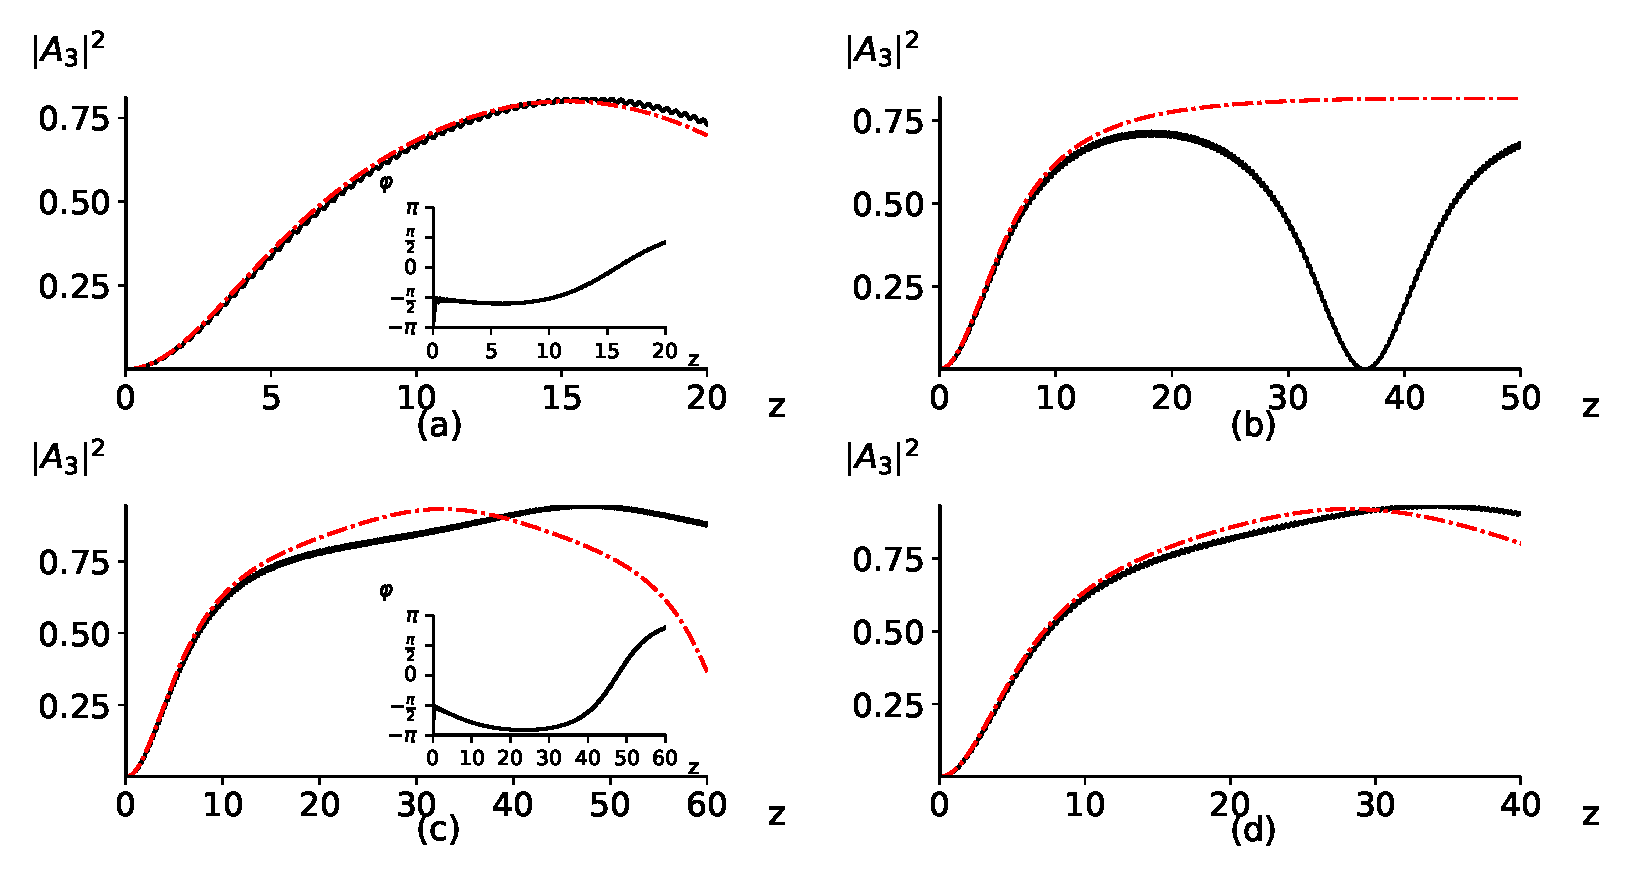
\includegraphics[width=0.8\linewidth]{CG_0.eps}  
\caption{ The TH intensity evolution computed on the base of both original problem (solid line) and the analytical solution of the modified problem (dashed-dotted line) at $\Delta_{31}k=0$ (a), $-0.05979923575$ (b), $-0.054$ (c), $-0.05$ (d).}
\label{fr:1}
\end{figure}

The insets in  Fig. \ref{fr:1}a, c confirms also the partial compensation of the phase nonlinear incursion by the phase mismatching $\Delta_{31}k$. The energy conversion from FW to TH occurs if the phase difference $\varphi$ is negative. In Fig. \ref{fr:1}a this takes place if the distance of laser pulse interaction is less than 15 dimensionless units. Meanwhile, that distance is about $z=45$ in Fig. \ref{fr:1}c. Both mentioned sections of z-coordinate corresponds to the phase difference equal  $\varphi=0$.

Let's note that with increasing power density of the incident pulse it is necessary accounting for the cubic non-linear response of a medium:  $\alpha \ne 0$ in \eqref{eq:ref1}.  The solution of the corresponding equations shows, that in this case choosing incident FW power density as well as the phase mismatching between FW and TH 

\begin{equation}
\label{eq:coef}
\begin{aligned}
\alpha=\frac{3\gamma^2}{2\Delta_{21}k},\\  \Delta_{31}k=-\frac{3\gamma^2}{2\Delta_{21}k},
\end{aligned}
\end{equation}
which corresponds, for example, to $q=-1.5$ ($\alpha=0.075,\,\Delta_{31}k=-0.075$ for $\gamma=1,\,\Delta_{21}k=20$), one can eliminate all negative influence of  self- and cross-modulation of interacting waves on the THG efficiency. In physical variables, the first equality is written as follows

\begin{equation}
\label{eq:coef1}
\begin{aligned}
&\chi^{(3)}=(4\pi(\chi^{(2)})^2k Z_n)/(3n^2\Delta_{21}{k}),
\end{aligned}
\end{equation}
here $\Delta_{21} k$ is dimensionless one. So, taking into account $\chi^{(2)}$ from Table \eqref{tab:2}, and $\chi^{(3)}\approx 2-6 10^{-22} m^2/V^2$ from \cite{bib:gan}, and wave-number as $k\approx 2\pi 10^6 m^{-1}$, $ and  n\approx 1.5$ for KDP crystal, we obtain that
$$
\Delta_{21}k\approx 10-30,
$$
which is close to value that we use in computer simulation.  In this case, the TH intensity, derived from the modified problem, varies as
$$
p_3(z)=\frac{\left(\frac{3\gamma^2 z}{2\Delta_{21}k}\right)^2}{1+\left(\frac{3\gamma^2 z}{2\Delta_{21}k}\right)^2}.
$$
It means that THG efficiency turns to $100\%$ as $  \frac{3\gamma^2 z}{2\Delta_{21}k}\rightarrow\infty$. 

\subsection*{SOD influence on the frequency tripling}

Below we discuss an influence of the SOD on the frequency up-conversion efficiency if the incident  pulse at FW possesses Gaussian shape 
\begin{equation}
A_{10}(t)=A_{01}e^{-(t-0.5L_t)^2},
\end{equation}
where \(A_{01}\) is equal to unity due to chosen dimensionless parameters, and the phase matching between TH and FW (\(\Delta_{31}k=0\)) as well as  group velocity matching (\(\nu_{21}=\nu_{31}=0\)) between interacting waves occur. We compare the computer simulation results obtained using the original problem \eqref{eq:ref1} and the modified problem \eqref{eq:main2} to demonstrate both a validity of the analytical consideration and a possibility for the high efficient THG achievement. It is important that a pulse at the trebled frequency possesses a smooth shape of  and its smooth broadened spectrum.

 
It should be emphasized that below the solution of the problem \eqref{eq:ref1}-\eqref{eq:first} is depicted as a solid line while the solution of the modified problem  \eqref{eq:main2}-\eqref{eq:ini2} is shown as a dotted line.  Numbers \(1,\,2,\,3\) in the Figs. denote FW, SH, and TH, respectively. In some cases, we also demonstrate the applicability of the analytical solution that is depicted as a dashed line. We pay a special attention to the pulses spectra and depict the initial spectrum distributions as well as the FW initial pulse shape in some Figs. using the solid line with triangles.


\paragraph*{Normal dispersion $(D_j<0)$ of a medium at FW wavelength }
\label{par:nor}
We note that in our notations a negative value of the dimensionless SOD coefficient corresponds to the normal dispersion of a medium. Below we consider the frequency tripling of the incident pulse with wavelength \(\lambda=800\,nm\) and  duration  \(100fs\) and propagating in a BBO crystal. In Fig. \ref{fr:c1_1}a-c the pulse shapes are depicted for the frequency up-conversion at the phase mismatching between SH and FW equaling \(\Delta_{21}k=20\) . It should be stressed that a positive sign of phase mismatching \(\Delta_{21}k\) corresponds to the FW pulse compression if it propagates in a medium with the normal SOD and the THG is not under consideration.

We see a good coincidence between the FW and TH pulse shapes, computed  using the original problem and the modified one, until the propagation distance \(z=13\) (Fig. \ref{fr:c1_1}a-f) . In this section the TH intensity is enough high: it achieves \(0.75\) dimensionless units at the pulse center. Despite a medium possesses, the THG accompanies by the spectral broadening of  both pulses in comparison with the incident FW pulse spectrum. Therefore, it is possible for further compression of the TH pulse (Fig. \ref{fr:c1_1}e). Wee see smooth spectrum of the TH \ref{fr:c1_1}d) meanwhile the FW pulse spectrum has two additional local minimums, which appear approximately in the vicinity of section 10 and it means that the sub-pulses appears at the FF (Fig. \ref{fr:c1_1}b). Under further propagation they lead to growing FW intensity with increasing  propagation distance (Fig. \ref{fr:c1_1}c,e). As a result, the conversion efficiency in the end of the propagation distance achieves \(51\%\) (\ref{fr:c1_1}f).

 We also want to note that the analytical solution perfectly describes the waves interaction until the section \(z=7.5\). Then we see that the FW pulse self-focusing and TH efficiency, predicted by the theory, are slightly higher than the corresponding values obtained from computer simulation results. Nevertheless, the equation \eqref{eq:main2} correctly describes a presence of the effective cubic non-linearity under waves interaction occurring at the cascading SHG. 
 
\begin{figure}[h!] 
\centering 
\includegraphics[width=\linewidth]{Cascade1_1-2}  
\caption{Pulse shapes in the sections \(z=7\) (a), \(10\) (b), \(13\) (c), and FW and TH spectra in the section \(z=13\) (d); pulse intensities evolution at their centers (e, g) and the frequency conversion efficiency evolution (f, h) along \(z\)-coordinate computed for the parameters $\gamma=1,\,  D_1=-0.0032,\, D_2=-0.0083,\, D_3=-0.0199$ and \,$\Delta_{21} k=20$ (e, f), -20 (g,h). Solid lines with triangles refer to incident pulse FW and its spectrum. Solid lines denote the original   problem solution; dotted lines --  the solution of modified problem, dashed lines -- the analytical solution} 
\label{fr:c1_1}
\end{figure}

\textcolor{ForestGreen}{In contrast to the long pulse duration approximation, the sign of $\Delta_{21}k$ influences on the frequency conversion process. So, } if the sign of the phase mismatching between FW and SH is negative (\(\Delta_{21}k=-20\)), then the energy conversion from the FW to TH also occurs with high efficiency (Fig.\ref{fr:c1_1} g-h). However, this sign of the phase mismatching corresponds to the FW pulse decompression due to induced cubic nonlinear response in a medium with a normal dispersion. As a result, the pulse duration of the FW and TH is greater than those at the positive phase mismatching (compare Fig. \ref{fr:c1_1}g-h and Fig.\ref{fr:c1_1}a-f). Nevertheless, a bandwidth of the TH pulse spectrum is also greater than those for the FW incident pulse. The energy conversion efficiency reaches the value of about \(68\%\) at increased crystal length in comparison with the previous case: a length of the current crystal  must be about \(3\,cm\). Other features of the THG are similar to the frequency up-conversion at the positive phase mismatching between the FW and TH. We can see also that the modified equations describe the interaction of waves with high accuracy.

\paragraph*{Anomalous dispersion $(D_1>0) $ of a medium at FW wavelength}
\label{par:an}

Let us briefly discuss the THG in a medium possessing anomalous dispersion at the frequency of FW. For example, this occurs  if the incident pulse with duration  \(100fs\) and wavelength \(1064nm\) propagates in KDP crystal. At the positive phase mismatching between FW and SH  (\(\Delta_{21}k>0\)), the FW pulse decompresses  and  of the pulse at trebled frequency compresses at their propagation. In this case, the efficiency of FW energy conversion to the TH energy achieves about \(60\%\) in the section \(z=15\) (Fig. \ref{fr:c1_11}a-d). The THG is accompanied by  TH pulse smooth shape and broadening its  spectrum in comparison with the incident pulse spectrum at the FF. In turn, the FW pulse shape has three intensity maximums and possesses smaller intensity at the pulse center in comparison with its value occurring at the pulse propagation in a medium possessing the normal dispersion at the FF. Nevertheless, we can see in Fig. \ref{fr:c1_11}b that the FW pulse spectrum is broadened also.

\begin{figure}[h!] 
\centering 
\includegraphics[width=0.9\linewidth]{Cascade1_11-12}  
\caption{Pulse shapes (a, e), their spectra (b, f) in the section \(z=15\) (a, b), 30 (e, f); pulse intensities evolution at their center (c, g) and the frequency conversion efficiency evolution (d, h) along \(z\)-coordinate computed for the parameters  $\gamma=1,\,  D_1=0.0006,\, D_2=-0.0035,\, D_3=-0.0062$ and  $\Delta_{21} k=20$ (a-d), -20 (e-h). \, Solid lines denote the solution of the original problem; dotted lines -- solution of the modified problem. 
}
\label{fr:c1_11}
\end{figure}

If the phase mismatching between FW and SH is negative (\(\Delta_{21}k<0\)), then the pulse compression at FF occurs, and decompression of the SH and TH pulses is observed. This leads to high-effective THG (Fig.\ref{fr:c1_11}e-h): more than \(80\%\) of the FW energy converts to the TH wave in the section  $z=30$ of a medium. However, the TH intensity is less than its value at the positive phase mismatching \(\Delta_{21}k\). Nevertheless, the TH spectrum is smooth and  broadened essentially.
\section*{Conclusion and remarks}

We have proposed a new physical scheme of THG based on cascading SHG, which leads to observing of the non-linear processes inherent  cubic nonlinear response. Therefore, the high-effective frequency tripling is possible for laser pulse or beam with the incident power density at which  the quadratic nonlinear response is observed.   A necessary length of a crystal, at which an efficient THG occurs, depends on the phase mismatching between the SH and FW and can be changed from 1.0 cm to 20 cm. It can be decreased with increasing power density of the incident pulse at FF.  THG process is accompanied by broadening  of the TH pulse spectrum that leads to possibility of  its further  compression.
Let's note that if the cubic susceptibility occurs then it is possible to compensate an influence of the pulse self- and cross-modulation on the frequency up-conversion by choosing the phase mismatching between interacting waves.


Using multi-scale method, we have derived the equations, named as  modified ones, describing frequency tripling due to cascading SHG and showed that they contain the terms responsible for phenomena inherent a medium with the cubic nonlinear response. Importantly, the equations do not contain the term responsible for the TH self-modulation that leads to enhancement of the up-conversion efficiency .  An analytical solution of the modified equations was developed in the framework of the long pulse duration approximation at using the derived integrals of motion. A validity of the modified equations is confirmed by computer simulation results obtained using the original Schr\"{o}dinger equations.

We have also investigated the influence of other parameters on the pulse interaction: SOD and the phase mismatching between TH and FW.  We shown that the high-effective  THG  is achieved for a medium possessing both anomalous and normal dispersion at the FF. Choice of the phase-mismatching between   FW and SH allows one to govern the regime of the laser pulse compression with FF. Because only quadratic nonlinear effects are required for THG through the cascading SHG then the effective frequency tripling  is possible for incident pulse with  picoseconds or nanoseconds duration.  

In our opinion, the proposed technique for optical frequency conversion can be used for other frequency conversion problems, such as Fourth Harmonic Generation or even Fifth Harmonic Generation or  a generation of wave with difference frequency.

\section*{Appendix: Derivation of the modified equations}
For demonstrating  appearance of the  induced cubic susceptibility of a medium due to cascading SHG, we use the multi-scale method \cite{bib:n24}, which was early applied in \cite{bib:n19} for demonstration of observing induced non-linearity similar Kerr effect and responsible for the pulse self-compression or its decompression  because of the  process under consideration. Because we consider a big phase mismatching between SH and FW: \(|\Delta_{21}k|>>1\), then the process of wave interaction possesses various space scales: in particular, a small scale, defined by big phase mismatching \(|\Delta_{21}k|\), and a long space scale defined by the dispersion lengths of the interacting pulses. 

Then let us introduce a small parameter \(\mu=\frac{1}{\Delta_{21}k}\) (for simplicity, we suppose that the phase mismatching has a positive sign) and introduce various scales along \(z\) coordinate: small scale equal to the inverse phase mismatching length: \(\xi=\frac{z}{\mu}\), and big longitudinal scales \(z_l=\mu^lz,\,l=0,1,2...\). Because of the big absolute value of the phase mismatching, the SHG efficiency is very low. Therefore, the complex amplitudes are expanded in a power series of \(\mu\):
\begin{equation}
\label{eq:exp}
\begin{aligned}
&A_1=U+\mu U_1 +\mu^2 U_2 +...,\\
&A_2=V+\mu V_1 + \mu^2 V_2 +...,\\
&A_3=W+\mu W_1 + \mu^2 W_2+....\\
\end{aligned}
\end{equation}
Obviously, the functions in \eqref{eq:exp} depend on all the variables \((t,\xi,z_l|l\ge0)\), and
the differential operators in terms of new variables take a form:
\begin{equation}
\label{eq:op}
\begin{aligned}
L_j&=\frac{\partial}{\partial z}+\nu_{j1}\frac{\partial}{\partial t}+iD_j\frac{\partial^2}{\partial t^2}=\frac{\partial \xi}{\partial z}\frac{\partial}{\partial \xi}+\sum\limits_{l=0}^{\infty}\frac{\partial z_l}{\partial z}\frac{\partial}{\partial z_l}+iD_j\frac{\partial^2}{\partial t^2}=\frac{1}{\mu}\frac{\partial}{\partial \xi}+\sum\limits_{l=0}^{\infty} \mu^l\frac{\partial}{\partial z_l}+iD_j\frac{\partial^2}{\partial t^2}\\
&=\frac{1}{\mu}\frac{\partial}{\partial \xi}+L_j^{0}+\mu\frac{\partial}{\partial z_1}+\mu^2 \frac{\partial}{\partial z_2}+...,j=1,2,3.
\end{aligned}
\end{equation}
Here, operator \(L_j\) is defined as 
\[L_j^{(0)}=\frac{\partial}{\partial z_0}+\nu_{j1}\frac{\partial}{\partial t}+ iD_j\frac{\partial^2}{\partial t^2}.\]

Then, substituting expansion \eqref{eq:exp} into the equation set \eqref{eq:refg} and collect terms, which are less than \(\mu^2\), we obtain the equations:
\begin{equation}
\label{eq:allset}
\begin{aligned}
&\frac{1}{\mu}\frac{\partial U}{\partial \xi}+L_1^{(0)}U+\mu \frac{\partial U}{\partial z_1}+\frac{\partial U_1}{\partial\xi}+\mu L_1^{(0)}U_1+\mu\frac{\partial U_2}{\partial \xi}+\\
+&i\gamma\left(U^*Ve^{-i\xi}+V^*We^{i\xi}+\mu((U^*V_1+U_1^*V)e^{-i\xi}+(V^*W_1+V_1^*W)e^{i\xi})\right)+O(\mu^2)=0,\\
&\frac{1}{\mu}\frac{\partial V}{\partial \xi}+L_2^{(0)}V+\mu \frac{\partial V}{\partial z_1}+\frac{\partial V_1}{\partial\xi}+\mu L_1^{(0)}V_1+\mu\frac{\partial V_2}{\partial \xi}+\\
+&i\gamma\left(U^2e^{i\xi}+2U^*We^{i\xi}+\mu(2UU_1e^{i\xi}+(U^*W_1+U_1^*W)e^{i\xi})\right)+O(\mu^2)=0,\\
&\frac{1}{\mu}\frac{\partial W}{\partial \xi}+L_3^{(0)}W+\mu \frac{\partial W}{\partial z_1}+\frac{\partial W_1}{\partial\xi}+\mu L_1^{(0)}W_1+\mu\frac{\partial W_2}{\partial \xi}+\\
+&3i\gamma \left(UVe^{-i\xi}+\mu(UV_1+U_1V)e^{-i\xi}\right)+i\Delta_{31}k(W+\mu W_1)+O(\mu^2)=0.
\end{aligned}
\end{equation}
The terms with respect to power of \(\frac{1}{\mu}\) allow us to write the equations:
\[\frac{\partial U}{\partial \xi}=\frac{\partial V}{\partial \xi}=\frac{\partial W}{\partial \xi}=0.\]
 Consequently, the functions \(U,\,V\) and \(W\) do not depend on fast changing coordinate \(\xi\), and they do not change at the small scale.

Next order \(O(1)\) of power \(\mu\) leads to the following equations:
\begin{equation}
\label{eq:fo}
\begin{aligned}
&L_1^{(0)}U+\frac{\partial U_1}{\partial\xi}+i\gamma(U^*Ve^{-i\xi}+V^*We^{i\xi})=0,\\
&L_2^{(0)}V+\frac{\partial V_1}{\partial \xi}+i\gamma(U^2e^{i\xi}+2U^*We^{i\xi})=0,\\
&L_3^{(0)}W+\frac{\partial W_1}{\partial \xi}+3i\gamma UVe^{-i\xi}+i\Delta_{31}kW=0.\\
\end{aligned}
\end{equation}
Because the first terms in these equations do not depend on \(\xi\) meanwhile other terms do depend on this variable, then one can separate equations into two parts. The first of them is written as
\begin{equation}
\label{eq:m1}
L_1^{(0)}U=L_2^{(0)}V=L_3^{(0)}W+i\Delta_{31}kW=0.
\end{equation}
The functions \(U_1,\,V_1,\,W_1\) can be found from the other parts by integrating \eqref{eq:fo} with respect to \(\xi\):
\begin{equation}
\label{eq:ford}
\begin{aligned}
&U_1=\gamma(U^*Ve^{-i\xi}-V^*We^{i\xi})+u_1(t,z_0,\,z_1...),\\
&V_1=\gamma(-U^2e^{i\xi}-2U^*We^{i\xi})+v_1(t,z_0,\,z_1...),\\
&W_1=3\gamma UVe^{-i\xi}+w_1(t,z_0,\,z_1...).\\
\end{aligned}
\end{equation}
Here \(u_1, v_1, w_1\) are the function of integration: they do not depend on \(\xi\). The equations with respect these functions are written further.

The order \(O(\mu)\) of the power serious leads to the equations:
\[\begin{aligned}
&\frac{\partial U_2}{\partial \xi}+L_1^{(0)}U_1+\frac{\partial U}{\partial z_1}+i\gamma((U^*V_1+U_1^*V)e^{-i\xi}+(V^*W_1+V_1^*W)e^{i\xi})=0,\\
&\frac{\partial V_2}{\partial \xi}+L_2^{(0)}V_1+\frac{\partial V}{\partial z_1}+i\gamma(2UU_1e^{i\xi}+(U^*W_1+U_1^*W)e^{i\xi})=0,\\
&\frac{\partial W_2}{\partial \xi}+L_3^{(0)}W_1+\frac{\partial W}{\partial z_1}+3i\gamma(UV_1+U_1V)e^{-i\xi}+\Delta_{31}kW_1=0.\\
\end{aligned}\]

Using the representation \eqref{eq:ford}, this set transforms into the form:
\begin{small}
\[\begin{aligned}
&\frac{\partial U_2}{\partial \xi}+\gamma(L_1^{(0)}(U^*V)e^{-i\xi}-L_1^{(0)}(V^*W)e^{i\xi})+i\gamma^2(U^*v_1e^{-i\xi}-V^2W^*e^{-2i\xi}+u_1^*Ve^{-i\xi}+V^*w_1e^{i\xi}+v_1^*We^{i\xi})=\\
&-\left(\frac{\partial U}{\partial z_1}+i\gamma^2(-|U|^2U-3U^{*2}W+4U|V|^2-2U|W|^2)\right)-L_1^{(0)}u_1,\\
&\frac{\partial V_2}{\partial \xi}-\gamma(L_2^{(0)}(U^2)e^{i\xi}+2L_2^{(0)}(U^*W)e^{i\xi})+i\gamma^2(-2UV^*We^{2i\xi}+2Uu_1e^{i\xi}+2UV^*We^{i\xi}+2u_1^*We^{i\xi}+2U^*we^{i\xi})=\\
&-\left(\frac{\partial V}{\partial z_1}+2i\gamma^2(4|U|-|W|^2)V\right)-L_2^{(0)}v_1,\\
&\frac{\partial W_2}{\partial \xi}+3\gamma L_3^{(0)}(UV)e^{-i\xi}+3i\gamma^2(Uv_1e^{-i\xi}+U^*V^2*e^{-2i\xi}+u_1V_1e^{-i\xi})+3i\Delta_{31}k\gamma UVe^{-i\xi}=\\
&-\left(\frac{\partial W}{\partial z_1}-3i\gamma^2(U^3+2|U|^2W+|V|^2W)\right)-L_1^{(0)}w_1-i\Delta_{31}kw_1.\\
\end{aligned}\]
\end{small}
As above we can state that the right-hand sides of the equations must be equal to zero because they do not depend on \(\xi\) in contrast to the left-hand sides of the equations. Thus, we write the equations
\[\begin{aligned}
&\frac{\partial U}{\partial z_1}+i\gamma^2(-|U|^2U-3U^{*2}W+4U|V|^2-2U|W|^2)=-L_1^{(0)}u_1,\\
&\frac{\partial V}{\partial z_1}+2i\gamma^2(4|U|^2-|W|^2)V=L_2^{(0)}v_1,\\
&\frac{\partial W}{\partial z_1}-3i\gamma^2(U^3+2|U|^2W+|V|^2W)=L_3^{(0)}w_1+i\Delta_{31}kw_1.\\
\end{aligned}\]
Because the functions \(u_1,\,v_1,\,w_1\)  belong to order \(O(\mu)\) (see \eqref{eq:ford} ) meanwhile the functions \(U,\,V,\,W\) belong to order \(O(1)\), then we can once again separate the obtained equation into two parts: 
\begin{equation}
\label{eq:mai}
\begin{aligned}
&\frac{\partial U}{\partial z_1}+i\gamma^2(-|U|^2U-3U^{*2}W+4U|V|^2-2U|W|^2)=0,\\
&\frac{\partial V}{\partial z_1}+2i\gamma^2(4|U|^2-|W|^2)V=0,\\
&\frac{\partial W}{\partial z_1}-3i\gamma^2(U^3+2|U|^2W+|V|^2W)=0.\\
\end{aligned}
\end{equation}
 Consequently, the equations
\begin{equation}
\begin{aligned}
&L_1^{(0)}u_1=0,\
&L_2^{(0)}v_1=0,\
&L_3^{(0)}w_1+i\Delta_{31}kw_1=0\
\end{aligned}
\end{equation}
are valid.

Finally, after returning to original variables (\(\xi=\Delta_{21}kz,\,z_0=z,\,z_1=z/\Delta_{21}k,\,\frac{\partial}{\partial z}=\Delta_{21}k\frac{\partial}{\partial \xi}+\frac{\partial}{\partial z_0}+\frac{1}{\Delta_{21}k}\frac{\partial}{\partial z_1}+O(\Delta_{21}k^{-2})\)), we obtain the following set of equations:
\begin{equation}
\label{eq:main}
\begin{aligned}
&\frac{\partial U}{\partial z}+iD_1\frac{\partial^2 U}{\partial t^2}-i\frac{\gamma^2}{\Delta_{21} k}(|U|^2U+3U^{*2}W-4U|V|^2+2U|W|^2)=0,\\
&\frac{\partial V}{\partial z}+\nu_{21}\frac{\partial V}{\partial t}+iD_2\frac{\partial^2 V}{\partial t^2}+2i\frac{\gamma^2}{\Delta_{21} k}(4|U|^2-|W|^2)V=0,\\
&\frac{\partial W}{\partial z}+\nu_{31}\frac{\partial W}{\partial t}+iD_3\frac{\partial^2 W}{\partial t^2}-3i\frac{\gamma^2}{\Delta_{21} k}(U^3+2|U|^2W+|V|^2W)+i\Delta_{31}kW=0\\
\end{aligned}
\end{equation}
with respect to \(U,V,W\), and the functions \(u_1,v_1,w_1\) are the solution of the linear Schr\"{o}dinger equations:
\begin{equation}
\label{eq:main_2}
\begin{aligned}
&\frac{\partial u_1}{\partial z}+iD_1\frac{\partial^2 u_1}{\partial t^2}=0,\\
&\frac{\partial v_1}{\partial z}+\nu_{21}\frac{\partial v_1}{\partial t}+iD_2\frac{\partial^2 v_1}{\partial t^2}=0,\\
&\frac{\partial w_1}{\partial z}+\nu_{31}\frac{\partial w_1}{\partial t}+iD_3\frac{\partial^2 w_1}{\partial t^2}+i\Delta_{31}kw_1=0,\\
\end{aligned}
\end{equation}
and the expansion series \eqref{eq:exp} transforms into the following form:
\begin{equation}
\label{eq:exp2}
\begin{aligned}
&A_1=U+\frac{1}{\Delta_{21}k}\left(\gamma(U^*Ve^{-i\Delta_{21}kz}-V^*We^{i\Delta_{21}kz})+u_1\right),\\
&A_2=V+\frac{1}{\Delta_{21}k}\left(-\gamma(U^2+2U^*W)e^{i\Delta_{21}kz}+v_1\right),\\
&A_3=W+\frac{1}{\Delta_{21}k}\left(3\gamma UVe^{-i\Delta_{21}kz}+w_1\right).\\
\end{aligned}
\end{equation}

Let's stress that without taking into account the wave with trebled frequency (\(A_3=W=w_1=0\)),  the equations \eqref{eq:main} -  \eqref{eq:exp2} reduce to the corresponding ones, derived in \cite{bib:n19}.

As we analyze the THG, then we believe that  the  SH and TH is absence in the input section of a medium. Therefore, the complex amplitudes \(A_2\) and \(A_3\) are equal to zero in this section. This results in the following conditions with respect to functions  \(U,\,V,\,W\):

\begin{equation}
\label{eq:ini3}
U|_{z=0}=A_1|_{z=0}=A_{10}(t),\,
V|_{z=0}=A_2|_{z=0}=0,\,
W|_{z=0}=A_3|_{z=0}=0.
\end{equation}
and to functions \(u_1,\,v_1,\,w_1\):
\begin{equation}
\label{eq:ini4}
 u_1|_{z=0}=w_1|_{z=0}=0,\, v_1|_{z=0}=\gamma A_{10}^2(t),
\end{equation}
respectively. At writing these conditions we  compare the corresponding terms in a series with respect to the small parameter \((\Delta_{21}k)^{-1}\) in \eqref{eq:exp2}. Since the initial distributions of the complex amplitudes \(A_j,\,j=1,2,3\) do not contain the terms at \((\Delta_{21}k)^{-1}\), then the corresponding terms in \eqref{eq:exp2} should be chosen equal to zero. Then the equations sets \eqref{eq:main}, \eqref{eq:main_2} reduce to the equations \eqref{eq:main2}. The reason is that the SH amplitude \(V\) equals zero ( \(V\equiv0\) ) due to both its initial condition \eqref{eq:ini3} and its including in all terms belonging to the second equation of the equations set \eqref{eq:main}. The same analysis shows that \(u_1\equiv0,\,w_1\equiv0\). Therefore, the representation \eqref{eq:exp2} reduces to the representation \eqref{eq:exp3}.
\subsection*{Acknowledgements}
D.M.K. and M.V.F. thank the Russian Science Foundation (Grant 19-11-00113)

\subsection*{Data availability}
The authors declare that all data supporting the findings of this study are available
within this article and its Supplementary Information files.

\subsection*{Code availability}
The custom computer code used to analyse and model the observational data here is available from the corresponding author on request, for the purpose of repeating 
the published results only.

\subsection*{Authors Contributions}
V.A.T. has proposed an original idea and method for investigation; D.M.K. and M.V.F. have implemented the theoretical analysis; D.M.K. has made the computer simulations; V.A.T., D.M.K. have taken parts in the results discussing and the paper writing.

\subsection*{Competing interests}
The authors declare no competing interests.

\subsection*{Correspondence and request for materials}
should be addressed to V.A.T. (trofimov@scut.edu.cn)


%\clearpage

\bibliographystyle{elsarticle-num}
\bibliography{sample}
\end{document} 